% !TeX document-id = {50f0f04c-d5f8-4417-bb49-0e71ddd7bfde}
% !TeX TXS-program:bibliography = txs:///biber

\documentclass[conference]{IEEEtran}
%\IEEEoverridecommandlockouts
% The preceding line is only needed to identify funding in the first footnote. If that is unneeded, please comment it out.
%\usepackage{cite}
\usepackage{amsmath,amssymb,amsfonts}
\usepackage{algorithmic}
\usepackage{graphicx}
\usepackage{textcomp}
\usepackage{xcolor}
\usepackage{tikz}
\usetikzlibrary{arrows.meta}
\usetikzlibrary{chains}
\usepackage{fontawesome5}
\usepackage{enumitem}
\usepackage{hyperref}
\usepackage[%
  bibstyle=ieee,
  citestyle=numeric,
  isbn=true,
  doi=false,
  sorting=none,
  url=true,
  defernumbers=true,
  bibencoding=utf8,
  backend=biber
]{biblatex}
\addbibresource{bibliography.bib}
%\usepackage{siunitx}

%% TODONOTES
\paperwidth=\dimexpr \paperwidth + 6cm\relax
\oddsidemargin=\dimexpr\oddsidemargin + 3cm\relax
\evensidemargin=\dimexpr\evensidemargin + 3cm\relax
\marginparwidth=\dimexpr \marginparwidth + 3cm\relax
\usepackage{todonotes}


% Key-system

\newcommand{\ptpKeyPrefix}{}
\newcommand{\ptpKey}[1]{\pgfkeysifdefined{\ptpKeyPrefix/#1}{\pgfkeysvalueof{\ptpKeyPrefix/#1}}{0}}
\newcommand{\fTime}[1]{#1\,\textmu{}s}
\newcommand{\fTimeKey}[1]{\fTime{\ptpKey{#1}}}
\newcommand{\fTimeMath}[2][0]{\fTime{\fpeval{round(#2, #1)}}}
\newcommand{\fRatio}[2][0]{\fpeval{round(#2, #1)}$\times$}
\newcommand{\fPercentage}[2][0]{\fpeval{round(100*(#2), #1)}\%}
\newcommand{\fRelative}[2][0]{\fpeval{round(100*(#2)-100, #1)}\%}

\begin{document}

\title{Telling the Time: Modern-Day Complications}
%\thanks{Identify applicable funding agency here. If none, delete this.}

\author{\IEEEauthorblockN{Vincent Bode}
\IEEEauthorblockA{\textit{Department of Computer Science} \\
\textit{Technical University of Munich}\\
Munich, Germany \\
vincent.bode@tum.de}
\and
\IEEEauthorblockN{Arpan Gujarati}
\IEEEauthorblockA{\textit{Department of Computer Science} \\
\textit{University of British Columbia}\\
Vancouver, Canada \\
arpanbg@cs.ubc.ca}
%\and
%\IEEEauthorblockN{3\textsuperscript{rd} Given Name Surname}
%\IEEEauthorblockA{\textit{dept. name of organization (of Aff.)} \\
%\textit{name of organization (of Aff.)}\\
%City, Country \\
%email address or ORCID}
}

\maketitle

\textbf{Potential Targets:}

\begin{tabular}{p{5cm}l}
    Venue & Deadline\\
    \href{https://ieee-ims.org/document/ispcs-2024-call-papers}{Symposium on Precision Clock Synchronization for Measurement, Control, \& Communication} & 20.03.2024\\
    \href{https://2024.rtss.org/call-for-papers/}{RTSS} & 23.05.2024\\
    \href{https://2024.rtss.org/call-for-papers/}{SIGMETRICS} & 02.08.2023 (first of 3)\\
    \href{https://ieee-ims.org/document/i2mtc-2024-call-papers}{Instrumentation and Measurement Technology Conference} & 24.11.2023\\
\end{tabular}

\begin{abstract}
\end{abstract}

\begin{IEEEkeywords}
PTP, Time Synchronization, Fault Tolerance
\end{IEEEkeywords}


\section{Introduction}
\todo{Find places to insert the word ``real-time'' to solidify applicability to RTSS.}
%``Time is of the essence'', to many readers this might only be an idiom but the relevance of time throughout our daily lives, processes and systems is so ubiquitous that we frequently fail to appreciate its significance. While the phrase is said to have originated from the legal domain, time-criticality and the necessity of having a common notion of time permeates all sectors, from logistics and manufacturing in industry, to service-level objectives in service providers, emergency response in public healthcare systems, activities in people's day-to-day routines, and even to academia, as everybody perpetually works towards the next deadline. In computer systems and communications, time has been with us from the very beginnings, with its significance showing from the most basic synchronized digital circuits even to places where one might not expect, such as in the world's most pervasive digital cryptography deployment, the SSL/TLS PKI~\cite{ssl-client-warnings}.

Time is both ubiquitous and critical, no computer system today can run without it. With the availability of the internet, satellite communications and digital clocks, we take for granted that we can tell the time anywhere and anytime.
%
%Nowadays, with the availability of the internet, satellite communications and digital clocks, we often take for granted that we can tell the time anywhere and anytime. And for most human use cases, a rough estimate of the current time on the order of magnitude of seconds is perfectly sufficient.
%After all, sub-second granularity is irrelevant as people follow their daily schedules, and for project plans that span years or even decades a day or two more will not make a difference. \todo{colloquial/irrelevant}
However, in communications, real-time systems and circuitry, we operate on a scale where things are not so simple, with sub-nanosecond-level accuracies gaining significance in areas like networks and chip design~\cite{nanopu,sub-nanosecond-comms-design}.

Global Navigation Satellite Systems (GNNS), a classical application enabled by precision time-synchronization, relies on signal propagation delays to determine relative positioning~\cite{intro-to-gnss}.
High-quality location estimates hinge on accurate timing and -compensation mechanisms, so GNSS is frequently leveraged as a nanoscale clock source~\cite{gnss-location-and-time-advances,gnss-for-high-precision-timing}.
%Failure to compensate clock differences or even the presence of adversarial signals can quickly degrade the resulting location quality~\cite{gps-jamming}, but in general GNNS systems enjoy widespread popularity not only as a way of acquiring location estimates but also as a way of obtaining highly accurate estimates of time~\cite{gnss-location-and-time-advances,gnss-for-high-precision-timing}.
The precision incurs expense though, it requires dedicated hardware, strains limited power budgets, and inhibits e.g. indoor deployments.

Timing is also critical for fault-tolerant systems. Architectures such as double- or triple-modular lock-step redundancy~\cite{triple-modular-redundancy,triple-modular-redundancy-evaluation,triple-modular-lock-step-arm}, where algorithms are run independently on different machines to automatically detect and correct errors, rely on a common notion of time and deadlines to make progress even when a machine has failed. Such systems are found frequently in high-reliability and -availability applications such as aviation, where computer systems are relied on for controlling machinery with strict timing requirements.
%Failed safety-critical redundancy engineering has seen some infamous examples recently, with deadly Boeing 737-Max incidents prompting the introduction of new laws for flight control computer error resilience~\cite{boeing-requirements}\todo{better citation}.
\todo{@Arpan I removed the example, it's too much for the intro.}
Without a common notion of time, it would not be possible for resilient systems to judge internally missed deadlines correctly, thus preventing the system from providing proper error-detection and correction, voiding the fault-tolerance it was designed for.

However, time is not only critical in fault-tolerant systems, it pervades all distributed systems.
High-performance and datacenter computing are areas large amounts of resources are being spent on maximizing hardware utilization by reducing I/O or communications bottlenecks~\cite{hpc-understanding-bottlenecks, hpc-solving-io-bottleneck, hpc-diagnosing-io-bottlenecks}, and a common notion of time is a prerequisite enabling technology to effective profiling and optimization on distributed systems.
%The better the time source, the easier it becomes to perform efficient handovers by precise scheduling, thus improving overall performance and resource consumption.
Google and Facebook\todo{cite} have come up with time synchronization implementations based on the notion of windows of uncertainty that can be used to ensure transaction ordering across a distributed system without an application having to explicitly synchronize, a property useful not only to databases but also to real-time control, fault detection/mitigation and parallel data structures.
Time synchronization techniques also transfer to edge computing, where scheduling computation and communication to efficiently manage load can conserve power and connectivity resources, allowing applications to achieve more with less hardware.
Even large scale deployments like the internet cannot function without timing, as SSL/TLS cryptographic certificate validation, renewal of leases (DHCP) and caches (DNS, HTTP), and various other state machines built into systems and protocols (TCP, firewalls, etc.) all rely on clocks to function.

Clearly, clock synchronization is essential in almost all aspects of computing, and there is a broad range of accuracies that we need to keep time in. But to what degree we can truly rely on modern computer timekeeping in distributed embedded systems when failures affect correctness?
We need to evaluate what our systems are capable of and what sort of reliability guarantees they can provide for our algorithms to work with.
Especially in industrial and embedded computing/IoT, deployments are often characterized by dependability/redundancy requirements and a general necessity to conserve all types of resources to reduce costs, as well as their relative isolation regarding connectivity.
This sets it apart from more traditional computer timekeeping scenarios, where an external source of truth can be relied upon, here internal consistency is the primary motivation.
%Good timekeeping allows a reduction in the amount of comparatively resource-intensive manual synchronization required, which directly leads to cost savings, however a high level of trust in the clock is needed to ensure ordering correctness. Across distributed embedded systems, we can use local network time synchronization to achieve this, however the question of accuracy and dependability under adverse conditions is open.
Before we can trust a synchronization algorithm, we need to understand how it performs and what causes it to break, which is what we will be investigating throughout the rest of this paper.
%\todo{Need a part here on what we are actually doing.}
%\todo{Dependable embedded systems.}


We evaluate the performance and resilience of four implementations of prevalent time synchronization protocols for packet-switched Ethernet networks, including the Precision Time Protocol (PTP) and the Network Time Protocol (NTP), across four hardware testbeds, showing strengths and weaknesses in a variety of configurations. We offer the following contributions:

\begin{itemize}
    \item Development of a tool, PTP-Perf, for fair and comparable cross-vendor evaluation of multiple time synchronization protocols and implementations,
    \item Establishment of a baseline of observed time-synchronization performance on several hardware testbeds across four vendors,
    \item Evaluation of synchronization resilience against adverse conditions/faults and possibilities of mitigating risk of synchronization failure,
    \item Assessment of deployability/resource consumption on embedded platforms,
    \item Provide lessons-learned and best practices for configuring time-synchronization deployments for high reliability and availability.
\end{itemize}

To the best of our knowledge, with PTP-Perf we provide the first data collection and analysis tooling available open-source\todo{anonymize} that supports the empirical evaluation of multiple Ethernet-based time synchronization protocols and implementations across several embedded hardware testbeds with an explicit focus on dependability and fault-tolerance.
%We also make the data collection and analysis tooling available open-source\todo{anonymize} to enable future studies to generate comparable results.
%
The rest of this paper is structured into the following sections: Section~\ref{sec:background} covers time synchronization and PTP background, as well as related work, while Section~\ref{sec:failure_scenarios} looks at potential failure scenarios. Results are presented in Sections~\ref{sec:baseline} Baseline, \ref{sec:resource_contention} Resource Contention, \ref{sec:fault_tolerance} Fault Tolerance and \ref{sec:resource_consumption} Resource Consumption. Finally, we present some lessons learned and best practices in Section~\ref{sec:learnings_conclusion}.

%\section{Applications that Require Time}
%\label{sec:motivation}



\section{Time Synchronization \& PTP}

Over the years, many different algorithms and solutions to time synchronization across computer networks have been explored [cite]. In today's most widely deployed network stack for general purpose computing, IP, two protocols have established themselves as standard for time synchronization: the Network Time Protocol (NTP) for Wide Area Networks (WANs) and the Precision Time Protocol (PTP) for Local Area Networks (LANs) that require a greater degree of time synchronization precision. Both protocols are standardized and each have multiple implementations available at the time of writing. Alternatives also include SPTP, a simplified version of PTP developed by Meta that claims to offer comparable performance to PTP while reducing resource consumption [cite].

Because we are interested in evaluating time synchronization for dependable systems, we will focus on PTP as it is designed to be deployed in controlled environments such as a fault-tolerant control network. PTP has wide-spread adoption and also serves as a foundation for technologies such as IEEE Time Sensitive Networking (TSN).


\subsection{PTP -- Background and Architecture}

PTP operates across a network and has two types of endpoints: master nodes and slave nodes. A PTP master provides synchronization signals to the slaves (Figure \ref{fig:ptp-architecture}), which each use the synchronization signal in combination with a path delay estimate to determine an estimate of the local clock offset to the master clock, which is subsequently used to discipline the local clock to keep it synchronized with the master's clock. While the actual protocol is slightly more complex and includes additional messages for synchronization leases and state management, the two core message types are sufficient in principle to synchronize the system clocks. Note that it is assumed that the PTP master already has a high-quality clock source for the current time -- preferably an external source like an atomic clock or a GPS signal, but the master clock can also be obtained from e.g. a different PTP domain.

\begin{figure}
    \begin{tikzpicture}[client/.style={draw}, message/.style={midway, above, sloped, inner sep=0mm}, on grid]
        \node[client] (master) {PTP Master};
        \node[client, above=of master] (clock) {\faClock[regular]};
        \draw[thick, dotted] (master) -- (clock);

        \node[client, right=1.75cm of master] (switch) {\faNetworkWired};
        \draw[-Stealth] (master) -- (switch);

        \foreach \i in {1,...,3}{
            \node[client] (slave-\i) at (3.5, \i - 2) {PTP Slave};
            \draw[-Stealth] (switch) -- (slave-\i.west);
        }

        \begin{scope}[xshift=5.5cm, yshift=2cm]
            \node (master) at (0,0) {Master};
            \node (slave) at (2,0) {Slave};

            \draw[-] (master) -- ++(0, -3.75);
            \draw[-] (slave) -- ++(0, -3.75);

            \foreach \i in {0.5, 1, 1.5}{
                \draw[-Stealth] (0, -\i) -- ++(2, -0.5) node[message] {Sync};
            }

            \draw[-Stealth] (2, -2.5) -- ++(-2, -0.5) node[message] {Delay Req.} -- ++(2, -0.5) node[message, below, inner sep=0.5mm] {Delay Resp.};
        \end{scope}
    \end{tikzpicture}
    \caption{
        A PTP master provides a synchronization signal to a number of slaves so that they can keep their local clock synchronized to the master's clock (left). The clock synchronization relies on two types of signals (right): a periodic synchronization signal to distribute the current master time and the delay request/response to estimate the propagation delay.
    }
    \label{fig:ptp-architecture}
\end{figure}

\subsection{PTP Profiles}
PTP is built to be configurable, settings include anything from the underlying transport (unicast/multicast), the delay mechanism to use (end-to-end or peer-to-peer), message frequencies and leases, as well as rules to discipline the clock. To reduce the complexity of configuring PTP, several so-called profiles are available that provide default settings for the specific use-case. \todo{Provide example profiles} To conduct our evaluation, we use each vendor's default profile, as this profile is the one that runs on general purpose deployments without special configuration, and is therefore the one that most users will come in contact with.

\subsection{Synchronization Performance}
It is generally understood that network clock synchronization accuracy is a function of the signal propagation delay and its variance [cite]. A naive approach to clock synchronization that just sends a timestamp from the master to the slave would always be off by the propagation delay, but PTP uses path delay estimation to try and compensate for the propagation delay thus increasing the accuracy. In an ideal world where there is no packet delay variation, the propagation delay could be mitigated entirely, but in reality we have multiple software and hardware components, like the kernel, network stack and network hardware, that each introduce latency variability, which in turn worsens the performance of the delay compensation. Effects such as asymmetric latencies caused by uneven loads that cannot easily be compensated for further reduce the synchronization accuracy. Thus, limiting the packet delay variation becomes a primary concern when tuning for precision and dependability.

\subsection{Hardware Acceleration}

\begin{figure}
    \newcommand{\timestampClock}[1][100]{\textcolor{black!#1}{\faClock[regular]}}

    \begin{tikzpicture}[
        start chain=components going below,
        start chain=components2 going below,
        component block/.style={draw, minimum height=0.75cm},
        node distance=0cm,
    ]

            \begin{scope}[name prefix=stack1-, component/.style={component block, text width=3.5cm}]
                \node[on chain=components, component] at (0, 0) (PTP) {PTP Client \hfill \rotatebox{45}{\faStamp{}} \timestampClock{} \faEnvelope[regular]};
                \node[on chain=components, component] (Kernel) {Kernel \hfill \timestampClock[60] \faEnvelope[regular]};
                \node[on chain=components, component] (IP-Stack) {IP Stack \hfill \timestampClock[40] \faEnvelope[regular]};
                \node[on chain=components, component] (Hardware Queue) {Hardware Queue \hfill \timestampClock[30] \faEnvelope[regular]};
                \node[on chain=components, component] (NIC) {NIC \faEthernet \hfill \timestampClock[20] \faEnvelope[regular]};

                \node[above=of PTP] (title) {Software PTP};
            \end{scope}

            \begin{scope}[name prefix=stack2-, component/.style={component block, text width=3.5cm}]
                \node[on chain=components2, component] at (5.5, 0) (PTP) {\faEnvelope[regular] \hfill PTP Client};
                \node[on chain=components2, component] (Kernel) {\faEnvelope[regular] \hfill Kernel};
                \node[on chain=components2, component] (IP-Stack) {\faEnvelope[regular] \hfill IP Stack };
                \node[on chain=components2, component] (Hardware Queue) {\faEnvelope[regular] \hfill Hardware Queue};
                \node[on chain=components2, component] (NIC) {\faEnvelope[regular] \faClock[regular] \rotatebox{-45}{\faStamp{}}  \hfill \faEthernet{} NIC};

                \node[above=of PTP] (title) {Hardware PTP};
            \end{scope}

            \draw[Stealth-Stealth, very thick] (stack1-NIC) -- (stack2-NIC) node[midway, draw, fill=white] (network) {\faNetworkWired};

            \node[draw, dashed, below=0.25cm of network] (network-annotation) {\faClock[regular] $\rightarrow$ \faHistory{}\,\textsuperscript{\textbf{*}}};
            \draw[dotted] (network.south west) -- (network-annotation.north west);
            \draw[dotted] (network.south east) -- (network-annotation.north east);

    \end{tikzpicture}
    \caption{
        Timestamping for PTP messages when using software timestamping (left) and hardware timestamping (right). For software timestamping, the timestamp is generated inside the PTP client and traverses many layers in both egress and ingress, causing additional path delay and delay variation. With hardware timestamping, a timestamp is only added to the message just before it is written to wire by the NIC, thus ensuring a more up-to-date timestamp is sent to the network.\\
        \textsuperscript{\textbf{*}}Network hardware (switches, routers, etc.) also introduces queuing delays. Special PTP-aware hardware can compensate for its own delays to further improve timestamping quality.
    }
    \label{fig:ptp-sw-hw}
\end{figure}

Since delay variation is a primary concern, hardware techniques have been developed to reduce the variability. While PTP can run entirely in software, the path that packets need to traverse between two PTP clients not only includes several hardware components but also some software layers (Figure~\ref{fig:ptp-sw-hw} left). Each component along the path introduces latency and packet delay variation, deteriorating the signal quality. With the appropriate hardware support, message timestamps can instead be generated directly by the NIC driver/hardware (Figure~\ref{fig:ptp-sw-hw} right), which ensures that the timestamp is not affected by the layers above it. This increases the clock synchronization's resilience against interference from adverse conditions, such as high network-, CPU- or kernel load.
\newcommand{\safetyMargin}{1000$\times$}

\section{Failure Scenarios}
\label{sec:failure_scenarios}
\todo{Should this be a sub-section}

Having an accurate clock synchronization across a network of machines can be just a nice-to-have for some applications, but applications that need to rely on the accuracy of the clock to perform their work need better guarantees than just an estimate of the accuracy.
Resilience is a top priority when building dependable systems, and to ensure that a system can operate reliably engineers will often add safety margins to their systems so that deviations in components of the system will not cause complete system failure.
In the context of time synchronization, since estimating the offset between clocks in software is imprecise even after applying denoising techniques, and the actual offset is influenced by a range of environmental conditions, the margin needs to be sufficiently large.
The high level of uncertainty combined with high risk, major consequences of failure, and/or system criticality for certain application scenarios can merit safety factors of 5$\times$, 10$\times$ or beyond depending on the application scenario\todo{Would be nice to have something to cite here}.
Naturally, the exact factor varies between use-cases, but for the purpose of our analysis of determining what conditions can lead to failures, we show that even highly conservative safety margins (e.g. three orders of magnitude, \safetyMargin) over the baseline can be broken, reinforcing the necessity of careful consideration of possible causes of failure.
%Thus, for our testbed of Raspberry Pis, a failure constitutes any time when the measured clock offset exceeds 40\,\textmu{}s\todo{out-of-place: hardware not introduced.}\todo{Actually insert the baseline.}.

\subsection{Sources of Error}
\todo{Should this be listed as a contribution?}
Error can originate from 2 principal sources: either the clock fails to perform according to specifications, or PTP's ability to measure and compensate the difference between clock sources is degraded or disrupted entirely. To understand what constitutes a failure in a timing system, we need to consider the guarantees that a timing system is required to provide to be useful and how they might be broken.

\paragraph*{Invariants of Timing Sources} Many of the assumptions made when using a clock are made implicitly because they seem natural in the real world, and a surprising number of software systems rely on them perhaps without being specifically aware of it. Timing systems need to fulfill all the following invariants, ranked in decreasing order of importance:

\newcounter{errorConditions}
\begin{enumerate}[label=I\arabic*.]
    \item \textbf{Time flows forward.}\todo{@Arpan wants citations but as of now: Based on my understanding. Find if somebody has formalized this.} This is perhaps the most trivial assumption, and the one with the worst consequences when it is violated. Generally, software systems do not account for the possibility of time flowing backwards, and it can cause any number of cascading failures, with common ones including missed deadlines (in cyclic events) as well as data inconsistencies (through tasks being executed multiple times) and data loss (accidental overwriting of previously collected data, e.g. backups, based on timestamps). Due to the these risks, even minor backward time shifts can result in system stability issues.
    \item \textbf{Time passes continuously, it does not jump.} While systems expect time to pass, jumping too far into the future can result in load spikes through e.g. too many scheduled tasks arriving simultaneously or scheduled tasks being skipped entirely. For stability, direct modifications of a clock at system runtime should be avoided in order to avoid breaking any real-time constraints the system is trying to observe.
    \item \textbf{Time passes at a constant rate.} While this might seem like the most important constraint, it is actually the easiest one to bend without compromising the usefulness of the clock. No process is perfect, thus tolerance is always expected, and for clocks this means that a certain level of clock drift is specified in the data sheet. In fact, software is designed to cope with some amount of variance in the flow of time, as modern day systems are often too complex to schedule anything at a precise point in time. Making clocks tick slightly faster or slower can be used for synchronization with fewer stability implications (this is called a clock slew).
    \setcounter{errorConditions}{\value{enumi}}
\end{enumerate}

Even during our experiments, which were carefully designed to account for the unreliable telling of time, we ran into issues with all of the above since PTP inevitably needs to violate (potentially all of) these assumptions to synchronize the clocks when there is a difference. Correcting for this error is difficult when there is no second source of time to cross-validate with, which is why we eventually used an external time source for record-keeping. Generally, PTP implementations try to minimize disruptions by breaking the lowest priority invariant possible to keep clocks in sync, exploiting the fact that I3 is more of a soft requirement.

\paragraph*{Multiple Sources of Time}

When two or more clocks are at play, then another invariant arises:

\begin{enumerate}[label=I\arabic*.]
    \setcounter{enumi}{\value{errorConditions}}
    \item \textbf{Coherence between ordered readings of different clocks.} A reading of one clock that comes before another should always yield a timestamp smaller than or equal to the latter to allow comparing them to be useful. This is theoretically equivalent with obtaining the same arbitrary-precision timestamp when reading both clocks simultaneously, but this is not possible in practice. Since this condition cannot be perfectly fulfilled i.e. there is always a margin of error, the coherency is only considered to be violated when the order is not preserved even though the readings were further apart than the tolerance bound.
\end{enumerate}

Establishing and maintaining coherency is PTP's primary purpose, and maintaining invariant I4 does not have a fixed priority\todo{Find if somebody has formalized this}, it sometimes merits breaking I3, I2 or even I1. However, for synchronization to even become possible two preconditions need to be fulfilled. These are the two principal challenges that PTP has to solve:

\begin{enumerate}[label=P\arabic*.]
%    \setcounter{enumi}{\value{errorConditions}}

    \item \textbf{Clock difference can be measured.} The prerequisite to synchronizing two clocks is to be able to quantify the offset, which is difficult to do reliably across packet-switched networks with best-effort quality of service due to the inherent packet-delay variation present.
    \item \textbf{Clock difference can be corrected.} Even when a difference can be measured it does not automatically imply that it can be corrected. Modifying current time has system stability implications because it directly violates conditions I1-I3, so time synchronization programs frequently have rules in place limiting under what conditions which invariants may be violated.
\end{enumerate}

In order for two clocks to stay synchronized, both conditions need to be continuously fulfilled to prevent divergence from occurring, which would cause invariant I4 to break down.

\subsection{Consequences of Failing to Maintain Invariants}
A violation of any of these conditions is an error in the timing system that can propagate throughout the entire system.
In the case of the first three clock invariants, failures will cause local incoherence, potentially triggering cascading failure even in system components that do not interact across a network. On the other hand, problems with time synchronization prerequisites causes clocks to diverge (I4), which only becomes noticeable upon communication when the coherency breaks down.
While this might seem less troublesome, the entire point of deploying PTP is to provide reliable and high accuracy time synchronization so that algorithms can use time for distributed scheduling, so a failure to provide this invalidates the usefulness of PTP itself.

The importance of maintaining clock invariants can be easy to underestimate. While small errors seem negligible for most timekeeping use cases, multiple production outages have been linked to timekeeping failures.
%One common cause is the existence of the leap-second, which,
%, an extra second that occurs once every few years to keep the calendar in sync with the earth's rotation.
The leap-second, despite its small magnitude, has been known to cause problems with navigation/collision avoidance systems, dead/live-locks occurring in the Linux kernel, and multi-hour outages in financial transaction processing systems~\cite{leap-seconds-recap}.
Significant engineering work has gone into mitigations, e.g. employing a leap-smear~\cite{leap-second-google, leap-second-technical-aspects} to avoid a time jump (rationale: condition I3 is less important than I1/I2), but these have in turn caused other outages,
%, but imperfections in the mitigation systems have in turn caused synchronization failures leading to accidental time jumps of 10 years magnitude~\cite{leap-seconds-recap}, large enough to break even ``simple'' systems that we take for granted such as SSL.
%The leap-second is such a significant reliability problem that recently calls are being made to abolish it altogether rather than trying to deal with its consequences~\cite{leap-second-facebook-abolish}, a resolution which has since found its way into the definition of UTC~\cite{leap-second-resolution}.
%Thus, the leap-second was
eventually leading to complete abolishment of leap-seconds via an amendment to UTC~\cite{leap-second-resolution,leap-second-facebook-abolish}.
When even well-vetted software such as the Linux kernel has resilience issues with one-second breaks in timing invariants, one can expect the average user application to be much less robust still, and no amount of replication can mitigate this.

Throughout this study, we will determine what can be expected of network time protocols, when and under what conditions the invariants and prerequisites inevitably break down under adverse conditions, and what this means for the ability of applications to reliably leverage Ethernet-based time synchronization.
%\todo{Explicitly list what our 10x bound means for each invariant.}

%\begin{table}
%    \centering
%    \caption{Conditions that constitute a violation of the time source invariants, as per the defined \safetyMargin{} safety margin above the baseline.}
%    \begin{tabular}{crr}
%        Invariant & Raspberry-Pi& 2nd System\\
%        I1 & $\Delta{}t<0$& \\
%        I2& $\Delta{}t>40$\textmu{}s& \\
%        I3& --& \\
%        I4& $|t_{C1} - t_{C2}| > 40$\textmu{}s& \\
%    \end{tabular}
%    \label{tbl:invariant-violation-limits}
%\end{table}


\section{Related Work}

NTP vs. PTP~\cite{ntp-vs-ptp}.

Failures in PTP~\cite{ptp-failures}.

Byzantine Attacks on PTP~\cite{byzantine-ptp}. Internal attacks on PTP~\cite{ptp-internal-attacks}.

PTP Redundancy~\cite{ptp-redundancy}


\section{Methodology}

\subsection{Testbed -- Hardware and Software}

\subsection{PTP Lifecycle}

\begin{figure*}
    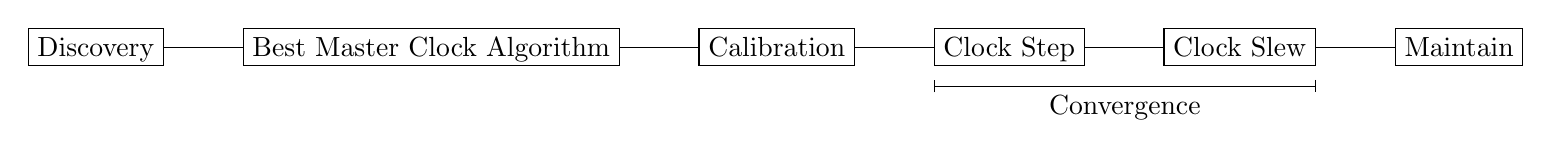
\begin{tikzpicture}[
        start chain=stages going right,
        stage/.style={
            draw, on chain=stages,
            every on chain/.style={join}, every join/.style={-Stealth}
        },
        text depth=0cm,
        ]
        \node[stage] {Discovery};
        \node[stage] {Best Master Clock Algorithm};
        \node[stage] (calibrate) {Calibration};
        \node[stage] (step) {Clock Step};
        \node[stage] (slew) {Clock Slew};
        \node[stage] {Maintain};

        \draw[Bar-Bar] ([yshift=-0.25cm]step.south west) -- ([yshift=-0.25cm]slew.south east) node[midway, below] {Convergence};
    \end{tikzpicture}
    \caption{Different stages in the PTP lifecycle that a PTP client traverses while synchronizing its clock. }
\end{figure*}

PTP clients traverse multiple stages in a lifecycle to synchronize their clock.

\section{Baseline Results}

\subsection{Baseline: The 1-to-1 benchmark}

We start by establishing a baseline for each tested system and vendor which we can later use as a comparison for different environment configurations. We collect data in 20 minute runs (corresponding to just above 1000 samples per run), while retaining the default setting of one synchronization and one measurement of the path delay per second, as our results suggest that a higher frequency does not significantly improve clock synchronization while negatively impacting the stability of the measurement\todo{This is stated but not shown. Do we need to show?}.

\begin{figure}
    \includegraphics[width=\linewidth]{res/generated/base/sample.pdf}
    \caption{A sample run of LinuxPTP in its default configuration. Because PTP uses path delay compensation, the clock synchronization accuracy is much better than the one-way path delay.}
    \label{fig:baseline_sample}
\end{figure}

Figure \ref{fig:baseline_sample} shows a sample run of the baseline for the LinuxPTP vendor. In order for collecting meaningful statistics, we apply some preprocessing to the collected profiles. \todo{Describe discarding calibration.}

\subsection{Vendors \& Systems}

\ptpperfLoadKeys{
    /ptpperf/base/rpi-4/ptpd/q5/.initial=6.016000000000001e-07,
    /ptpperf/base/rpi-4/ptpd/q50/.initial=7.395e-06,
    /ptpperf/base/rpi-4/ptpd/q95/.initial=4.5662000000000004e-05,
    /ptpperf/base/rpi-4/linuxptp/q5/.initial=5.2725e-07,
    /ptpperf/base/rpi-4/linuxptp/q50/.initial=5.0169999999999996e-06,
    /ptpperf/base/rpi-4/linuxptp/q95/.initial=1.50795e-05,
    /ptpperf/base/rpi-4/sptp/q5/.initial=2.08e-07,
    /ptpperf/base/rpi-4/sptp/q50/.initial=2.4485000000000004e-06,
    /ptpperf/base/rpi-4/sptp/q95/.initial=7.866249999999998e-06,
    /ptpperf/base/rpi-4/chrony/q95/.initial=4.808600000000004e-06,
    /ptpperf/base/rpi-4/chrony/q50/.initial=1.325e-06,
    /ptpperf/base/rpi-4/chrony/q5/.initial=1.1900000000000001e-07,
    /ptpperf/base/rpi-5/ptpd/q5/.initial=1.01e-07,
    /ptpperf/base/rpi-5/ptpd/q50/.initial=1.13e-06,
    /ptpperf/base/rpi-5/ptpd/q95/.initial=3.668349999999999e-06,
    /ptpperf/base/rpi-5/linuxptp/q95/.initial=8.790000000000001e-07,
    /ptpperf/base/rpi-5/linuxptp/q50/.initial=3.2600000000000003e-07,
    /ptpperf/base/rpi-5/linuxptp/q5/.initial=2.8000000000000003e-08,
    /ptpperf/base/rpi-5/sptp/q50/.initial=5.03e-07,
    /ptpperf/base/rpi-5/sptp/q95/.initial=1.6650000000000002e-06,
    /ptpperf/base/rpi-5/sptp/q5/.initial=4.6e-08,
    /ptpperf/base/rpi-5/chrony/q50/.initial=1.7600000000000001e-07,
    /ptpperf/base/rpi-5/chrony/q5/.initial=1.4000000000000001e-08,
    /ptpperf/base/rpi-5/chrony/q95/.initial=5.09e-07,
}


\begin{figure}
    \includegraphics[width=\linewidth]{res/generated/base/vendor_comparison.pdf}
    \caption{Median baseline performance for all vendors, across our two hardware testbeds (left) and magnified for only the Raspberry-Pi 5 cluster (right). Error bands represent the 5\textsuperscript{th} and 95\textsuperscript{th}, respectively.}
    \label{fig:baseline}
\end{figure}

\begin{table}
\centering
\caption{Baseline Values by Vendor and System}
\begin{tabular}{rrrrr}
           & \multicolumn{2}{c}{Med. Clock Offset} & \multicolumn{2}{c}{$P_{95}$ Clock Offset}\\
    System & LinuxPTP & PTPd & LinuxPTP & PTPd\\
    Raspberry-Pi 4 & \fTimeKey{linuxptp/median} & \fTimeKey{ptpd/median} & \\
\end{tabular}
\end{table}

\cmpSearchVendor{\ptpKey{base/rpi-4/\vendor/q50}}

A logical first step is comparing each vendor's baseline across the systems. Figure~\ref{fig:baseline} shows the four vendors on the Raspberry-Pi 4 and Raspberry-Pi 5 clusters. We observe that \fVendor{\cmpMaxArg} has the worst synchronization offset on both systems, with a median clock offset of \fTime[1]{\cmpMax} on the Raspberry-Pi 4 and \fTimeKey[1]{base/rpi-5/ptpd/q50} on the Raspberry-Pi 5.
%
%
\fVendor{\cmpMinArg}, on the other hand, has the best performance on both systems, with the clock offset estimate at just \fTime[1]{\cmpMin} and \fTimeKey[1]{base/rpi-5/chrony/q50}, respectively.
\todo{Both machines can not be Latex verified.}

\cmpSearch{\vendor}{ptpd,linuxptp,sptp,chrony}{\ptpKey{base/rpi-4/\vendor/q50}/\ptpKey{base/rpi-5/\vendor/q50}}

The most noticeable effect on the synchronization quality is the hardware, which is expected since the Raspberry-Pi 5 offers hardware timestamping while the Raspberry-Pi 4 does not. The advantage ranges from \fRatio{\cmpMin} for \fVendor{\cmpMinArg} to \fRatio{\cmpMax} for \fVendor{\cmpMaxArg}.

%\todo{
Advantages: \foreach \vendor in {ptpd,linuxptp,sptp,chrony}{\fRatio{\ptpKey{base/rpi-4/\vendor/q50}/\ptpKey{base/rpi-5/\vendor/q50}} }
%}

\cmpSearchVendor{\ptpKey{base/rpi-4/\vendor/q95}/\ptpKey{base/rpi-4/\vendor/q50}}%
Another aspect to notice is the difference between the median clock offset and the 95\textsuperscript{th} percentile. Without hardware support, this difference can be rather large and has a high spread (between \fRatio{\cmpMin} for the most stable vendor \fVendor{\cmpMinArg} and \fRatio{\cmpMax} for the least stable vendor \fVendor{\cmpMaxArg}),
whereas the magnitude is smaller when hardware support is offered on the Raspberry-Pi %
\cmpSearchVendor{\ptpKey{base/rpi-5/\vendor/q95}/\ptpKey{base/rpi-5/\vendor/q50}}%
(\fRatio[1]{\cmpMin} \fVendor{\cmpMinArg} -- \fRatio[1]{\cmpMax} \fVendor{\cmpMaxArg}).
This means that not only is the average performance improved, but the magnitude of outliers is reduced, which is especially important when considering the dependability aspect.

\subsection{Reproducibility}

\pgfkeys{
    /reproducibility/rpi-4/.cd,
    ptpd/min/.initial={5.3},
    ptpd/median/.initial={6.1},
    ptpd/max/.initial={24},
    linuxptp/min/.initial={4.2},
    linuxptp/median/.initial={5.1},
    linuxptp/max/.initial={6.0},
}
\renewcommand{\ptpKeyPrefix}{/reproducibility/rpi-4}


\begin{figure}
    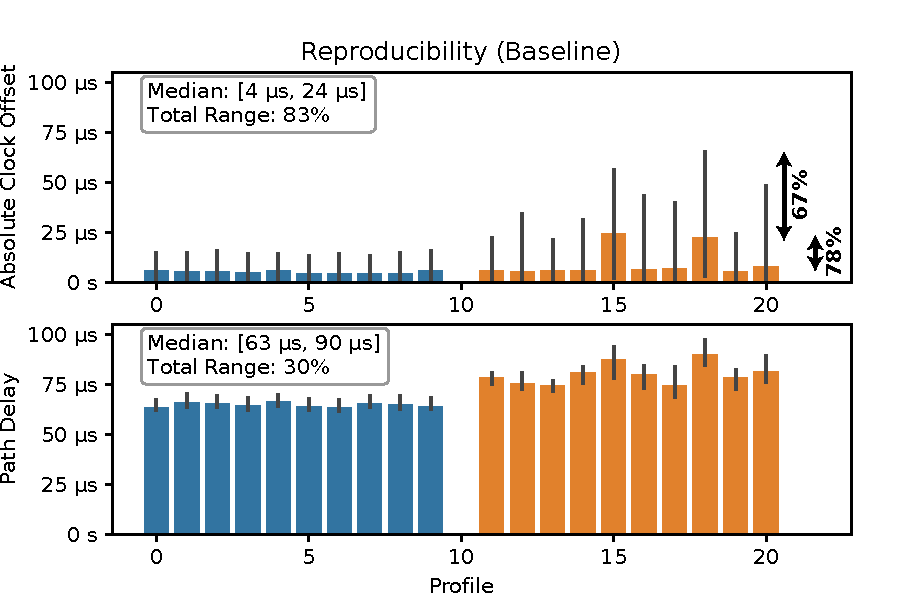
\includegraphics[width=\linewidth]{res/generated/base/key_metric_variance.pdf}
    \caption{Validating the baseline results by repeatedly measuring the baseline for both vendors on the Raspberry Pi 4 system. Top: The median absolute clock offset for each run, with error bars reaching from quantiles 0.05 to 0.95. Bottom: The same for the estimated path delay.}
    \label{fig:baseline_reproducibility}
\end{figure}

\newcommand{\numBaselineMeasurements}{10}
\newcommand{\baselineMinutesRuntime}{\numBaselineMeasurements*4*2*20}

The next question to be answered is how reproducible the baseline is. To evaluate this, we repeat the measurement of the baseline observations ten times for each vendor on each hardware platform (totaling in around \fpeval{round(\baselineMinutesRuntime/60)} hours of runtime and \fpeval{round(\baselineMinutesRuntime*60)} samples collected) and aggregate them. Between each measurement run, the entire cluster is restarted to ensure that no state is carried over, which would harm the independence of observations. Otherwise, the setup is left untouched and all that happens is that the PTP installation is started and stopped.

%Figure \ref{fig:baseline_reproducibility} shows the results. We observe that LinuxPTP produces significantly more stable results for both the clock offset estimation and the path delay, while PTPd shows more variance in median and 95-th quantile observed clock offset, while additionally being less sure about the path delay. A simple restart can suddenly cause the median latency to jump from the median \fTimeKey{ptpd/median} up to \fTimeKey{ptpd/max}, which corresponds to an increase of \fRatio{\ptpKey{ptpd/max}/\ptpKey{ptpd/median}} not only momentarily, but throughout an entire run. This already comes uncomfortably close to our safety factor of \safetyMargin, and we have not even started stressing the system yet. Fortunately, LinuxPTP produces a lot more stable results, with a smaller range of \fTimeKey{linuxptp/median} and \fTimeKey{linuxptp/max} between the median observed run and the worst observed run corresponding to just \fRelative{\ptpKey{linuxptp/max}/\ptpKey{linuxptp/median}}.




\printbibliography

\end{document}